% Options for packages loaded elsewhere
\PassOptionsToPackage{unicode}{hyperref}
\PassOptionsToPackage{hyphens}{url}
%
\documentclass[
]{article}
\usepackage{lmodern}
\usepackage{amssymb,amsmath}
\usepackage{ifxetex,ifluatex}
\ifnum 0\ifxetex 1\fi\ifluatex 1\fi=0 % if pdftex
  \usepackage[T1]{fontenc}
  \usepackage[utf8]{inputenc}
  \usepackage{textcomp} % provide euro and other symbols
\else % if luatex or xetex
  \usepackage{unicode-math}
  \defaultfontfeatures{Scale=MatchLowercase}
  \defaultfontfeatures[\rmfamily]{Ligatures=TeX,Scale=1}
\fi
% Use upquote if available, for straight quotes in verbatim environments
\IfFileExists{upquote.sty}{\usepackage{upquote}}{}
\IfFileExists{microtype.sty}{% use microtype if available
  \usepackage[]{microtype}
  \UseMicrotypeSet[protrusion]{basicmath} % disable protrusion for tt fonts
}{}
\makeatletter
\@ifundefined{KOMAClassName}{% if non-KOMA class
  \IfFileExists{parskip.sty}{%
    \usepackage{parskip}
  }{% else
    \setlength{\parindent}{0pt}
    \setlength{\parskip}{6pt plus 2pt minus 1pt}}
}{% if KOMA class
  \KOMAoptions{parskip=half}}
\makeatother
\usepackage{xcolor}
\IfFileExists{xurl.sty}{\usepackage{xurl}}{} % add URL line breaks if available
\IfFileExists{bookmark.sty}{\usepackage{bookmark}}{\usepackage{hyperref}}
\hypersetup{
  hidelinks,
  pdfcreator={LaTeX via pandoc}}
\urlstyle{same} % disable monospaced font for URLs
\usepackage[margin=1in]{geometry}
\usepackage{color}
\usepackage{fancyvrb}
\newcommand{\VerbBar}{|}
\newcommand{\VERB}{\Verb[commandchars=\\\{\}]}
\DefineVerbatimEnvironment{Highlighting}{Verbatim}{commandchars=\\\{\}}
% Add ',fontsize=\small' for more characters per line
\usepackage{framed}
\definecolor{shadecolor}{RGB}{248,248,248}
\newenvironment{Shaded}{\begin{snugshade}}{\end{snugshade}}
\newcommand{\AlertTok}[1]{\textcolor[rgb]{0.94,0.16,0.16}{#1}}
\newcommand{\AnnotationTok}[1]{\textcolor[rgb]{0.56,0.35,0.01}{\textbf{\textit{#1}}}}
\newcommand{\AttributeTok}[1]{\textcolor[rgb]{0.77,0.63,0.00}{#1}}
\newcommand{\BaseNTok}[1]{\textcolor[rgb]{0.00,0.00,0.81}{#1}}
\newcommand{\BuiltInTok}[1]{#1}
\newcommand{\CharTok}[1]{\textcolor[rgb]{0.31,0.60,0.02}{#1}}
\newcommand{\CommentTok}[1]{\textcolor[rgb]{0.56,0.35,0.01}{\textit{#1}}}
\newcommand{\CommentVarTok}[1]{\textcolor[rgb]{0.56,0.35,0.01}{\textbf{\textit{#1}}}}
\newcommand{\ConstantTok}[1]{\textcolor[rgb]{0.00,0.00,0.00}{#1}}
\newcommand{\ControlFlowTok}[1]{\textcolor[rgb]{0.13,0.29,0.53}{\textbf{#1}}}
\newcommand{\DataTypeTok}[1]{\textcolor[rgb]{0.13,0.29,0.53}{#1}}
\newcommand{\DecValTok}[1]{\textcolor[rgb]{0.00,0.00,0.81}{#1}}
\newcommand{\DocumentationTok}[1]{\textcolor[rgb]{0.56,0.35,0.01}{\textbf{\textit{#1}}}}
\newcommand{\ErrorTok}[1]{\textcolor[rgb]{0.64,0.00,0.00}{\textbf{#1}}}
\newcommand{\ExtensionTok}[1]{#1}
\newcommand{\FloatTok}[1]{\textcolor[rgb]{0.00,0.00,0.81}{#1}}
\newcommand{\FunctionTok}[1]{\textcolor[rgb]{0.00,0.00,0.00}{#1}}
\newcommand{\ImportTok}[1]{#1}
\newcommand{\InformationTok}[1]{\textcolor[rgb]{0.56,0.35,0.01}{\textbf{\textit{#1}}}}
\newcommand{\KeywordTok}[1]{\textcolor[rgb]{0.13,0.29,0.53}{\textbf{#1}}}
\newcommand{\NormalTok}[1]{#1}
\newcommand{\OperatorTok}[1]{\textcolor[rgb]{0.81,0.36,0.00}{\textbf{#1}}}
\newcommand{\OtherTok}[1]{\textcolor[rgb]{0.56,0.35,0.01}{#1}}
\newcommand{\PreprocessorTok}[1]{\textcolor[rgb]{0.56,0.35,0.01}{\textit{#1}}}
\newcommand{\RegionMarkerTok}[1]{#1}
\newcommand{\SpecialCharTok}[1]{\textcolor[rgb]{0.00,0.00,0.00}{#1}}
\newcommand{\SpecialStringTok}[1]{\textcolor[rgb]{0.31,0.60,0.02}{#1}}
\newcommand{\StringTok}[1]{\textcolor[rgb]{0.31,0.60,0.02}{#1}}
\newcommand{\VariableTok}[1]{\textcolor[rgb]{0.00,0.00,0.00}{#1}}
\newcommand{\VerbatimStringTok}[1]{\textcolor[rgb]{0.31,0.60,0.02}{#1}}
\newcommand{\WarningTok}[1]{\textcolor[rgb]{0.56,0.35,0.01}{\textbf{\textit{#1}}}}
\usepackage{graphicx,grffile}
\makeatletter
\def\maxwidth{\ifdim\Gin@nat@width>\linewidth\linewidth\else\Gin@nat@width\fi}
\def\maxheight{\ifdim\Gin@nat@height>\textheight\textheight\else\Gin@nat@height\fi}
\makeatother
% Scale images if necessary, so that they will not overflow the page
% margins by default, and it is still possible to overwrite the defaults
% using explicit options in \includegraphics[width, height, ...]{}
\setkeys{Gin}{width=\maxwidth,height=\maxheight,keepaspectratio}
% Set default figure placement to htbp
\makeatletter
\def\fps@figure{htbp}
\makeatother
\setlength{\emergencystretch}{3em} % prevent overfull lines
\providecommand{\tightlist}{%
  \setlength{\itemsep}{0pt}\setlength{\parskip}{0pt}}
\setcounter{secnumdepth}{-\maxdimen} % remove section numbering

\author{}
\date{\vspace{-2.5em}}

\begin{document}

Escribo acá algunos posibles ejercicios

\[\huge 🙈\]

En esta guía veremos cómo modelar una serie de datos observados usando:

\begin{enumerate}
\def\labelenumi{\arabic{enumi}.}
\item
  \textbf{Máximos por Períodos} y el \textbf{\emph{Teorema de
  Generalized Extreme Values (GEV)}}
\item
  \textbf{Excesos sobre Umbral} y el \textbf{\emph{Teorema de
  Generalized Pareto Distribution (GPD)}}
\end{enumerate}

Los datos se corresponden al dataset de \(\mathcal C\)arli
\texttt{{[}y\ acá\ iría\ descripción\ del\ dataset{]}}.

\begin{enumerate}
\def\labelenumi{\arabic{enumi}.}
\tightlist
\item
  Para máximos por períodos:
\end{enumerate}

\begin{quote}
usamos Gumbell como dijo Mariela? justificando que es el caso más común
y (tal vez) simple de analizar.

Mencionamos usos de los otros dos casos? maybe grafiquitos en imagen y
fin?
\end{quote}

\begin{enumerate}
\def\labelenumi{\arabic{enumi}.}
\tightlist
\item
  Para umbral
\end{enumerate}

\begin{quote}
Hay solo una, pero con parámetro = 0
\end{quote}

\begin{enumerate}
\def\labelenumi{\arabic{enumi}.}
\setcounter{enumi}{2}
\tightlist
\item
  Para ambos
\end{enumerate}

\begin{quote}
\begin{itemize}
\item
  Filtrar datos =\textgreater{} Ajustar F =\textgreater{} Devolver
  parámetros Maybe: Guardar matriz de var-cov =\textgreater{} calcular
  varianza del nivel de retorno
  \(Var(\hat z_p)\approx \nabla z_p^T \ V \ \nabla z_p\), donde V es la
  matriz de var-cov de los estimadores de cada parametro

  Capaz se pueda graficar el nivel de retorno en funcion del umbral, Y
  su varianza, para ver como varía a medida que tenemos menos datos en
  valores más extremos.

  Y como tengo tableta de dibujo, te hago un dibujito:
\end{itemize}

\begin{figure}
\centering
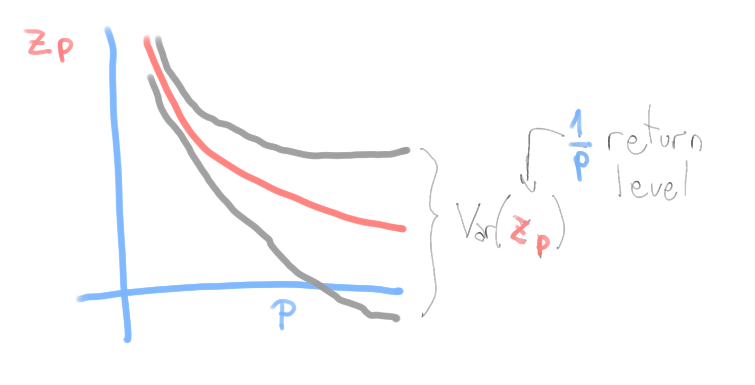
\includegraphics{../Imagenes/varianza-del-nivel-de-retorno.png}
\caption{varianza-del-nivel-de-retorno.png}
\end{figure}
\end{quote}

\hypertarget{intuicion-de-distribuciuxf3n-del-muxe1ximo.}{%
\subsubsection{Intuicion de distribución del
máximo.}\label{intuicion-de-distribuciuxf3n-del-muxe1ximo.}}

Sabemos que un histograma aproxima \emph{(de una forma burda)} la
función de densidad \(f(x)\) a partir de la cual se generaron los datos
\(x_1, x_2, \dots, x_n\), asumiendo que son \textbf{realizaciones} de
variables aleatorias \(X_1, X_2, \dots, X_n \ \text{iid}\) con
\(X_1 \sim f\)

\begin{Shaded}
\begin{Highlighting}[]
\NormalTok{gridx <-}\StringTok{ }\KeywordTok{seq}\NormalTok{(}\OperatorTok{-}\DecValTok{3}\NormalTok{,}\DecValTok{3}\NormalTok{, }\FloatTok{0.1}\NormalTok{)}
\KeywordTok{hist}\NormalTok{(}\KeywordTok{rnorm}\NormalTok{(}\FloatTok{1e5}\NormalTok{), }\DataTypeTok{prob=}\NormalTok{T, }\DataTypeTok{ylim=}\KeywordTok{c}\NormalTok{(}\DecValTok{0}\NormalTok{,}\FloatTok{0.45}\NormalTok{), }\DataTypeTok{col=}\StringTok{'steelblue'}\NormalTok{, }\DataTypeTok{main=}\StringTok{"Histograma de Datos ~ N(0,1)"}\NormalTok{)}
\KeywordTok{lines}\NormalTok{(gridx, }\KeywordTok{dnorm}\NormalTok{(gridx), }\DataTypeTok{lwd=}\DecValTok{3}\NormalTok{, }\DataTypeTok{col=}\StringTok{'orange'}\NormalTok{)}
\end{Highlighting}
\end{Shaded}

\includegraphics{Guia-1_files/figure-latex/unnamed-chunk-2-1.pdf}

En el problema de modelado de máximos, queremos encontrar una función
\(g(x)\) a partir de la cual se generaron los datos
\(\hat x_1, \hat x_2, \dots ,\hat x_m\), asumiendo que son
\textbf{realizaciones} de variables aleatorias
\(\hat X_1, \hat X_2, \dots, \hat X_m \ \text{iid}\) con
\(\hat X_1 \sim g\)

Siendo concretos, los datos que queremos modelar son:

\begin{itemize}
\item
  Los que sobrepasan algún umbral

  \begin{itemize}
  \tightlist
  \item
    ej: ``\(x_i\) mayores a 30'', ``\(x_i\) mayores al 95 percentil''
  \end{itemize}
\item
  Los máximos en un período (bloque) dado

  \begin{itemize}
  \tightlist
  \item
    ej: ``teniendo \(x_i\) diarios, quiero el mayor \(x_i\) de cada
    año''
  \end{itemize}
\end{itemize}

Llamamos \(\hat x_i\) a los \(x_i\) que cumplen su condición de
``\textbf{máximo}'' en cualquiera de los casos.

En otras palabras, solo estamos interesados en \textbf{la cola de la
distribución}.

\hypertarget{antes-de-pasar-al-siguiente-ejercicio}{%
\subsubsection{Antes de pasar al siguiente
ejercicio:}\label{antes-de-pasar-al-siguiente-ejercicio}}

\begin{quote}
¿Podés imaginar cómo resultaría un histograma de los \textbf{valores
máximos} \(\hat x_i\) que se encuentran \textbf{en la cola} de una
Normal(0,1) como la anterior, a medida que la cantidad de muestras
tiende a infinito?

¿Podés ver por qué ésto no es así? Qué sucede ``alrededor'' del umbral?
¿Por qué?
\end{quote}

\begin{quote}
\begin{quote}
\hypertarget{rta}{%
\subsubsection{RTA}\label{rta}}

Es razonable pensar que un histograma de los valores de la cola de una
Normal, será exactamente igual que recortar la cola de un histograma
``completo''.

Pero al tener un umbral que \textbf{descarta} los valores por debajo del
mismo, podemos ver cómo la probabilidad (área) de caer en un entorno de
\(u\) se redujo a la mitad

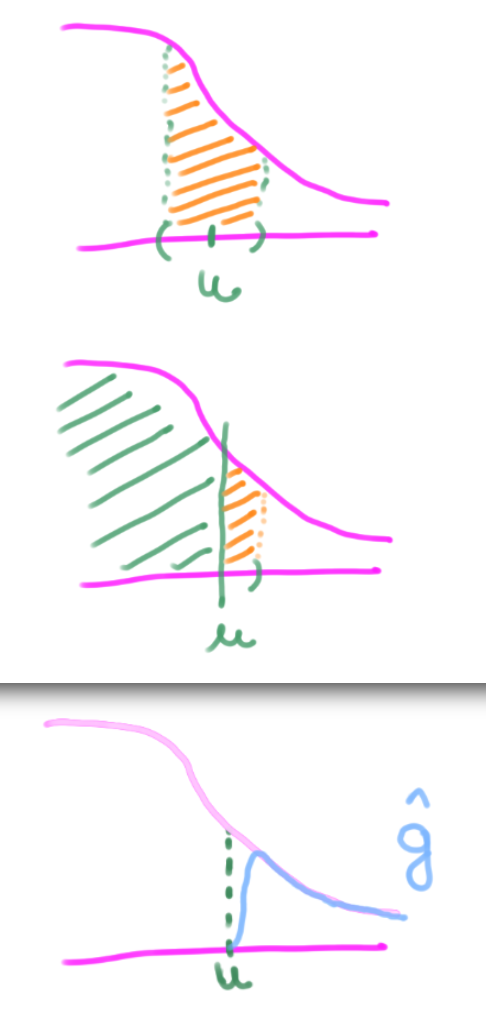
\includegraphics{../Imagenes/intro.png}
\end{quote}
\end{quote}

\hypertarget{ejercicio-1.}{%
\section{Ejercicio 1.}\label{ejercicio-1.}}

Realice un \textbf{histograma del percentil 90} como umbral de una
muestra \textbf{Normal estándar} de \texttt{1e5} elementos.

Agregue una curva de densidad estimada \(\hat g\) utilizando la función
\texttt{density} sobre los \textbf{datos del histograma}.

\hypertarget{rta-1}{%
\subsubsection{RTA}\label{rta-1}}

Realizamos un histograma de los datos por encima del umbral. Para
filtrarlos: \textgreater{}
\texttt{datos{[}datos\ \textgreater{}\ umbral{]}}

\begin{Shaded}
\begin{Highlighting}[]
\NormalTok{datos  <-}\StringTok{ }\KeywordTok{rnorm}\NormalTok{(}\FloatTok{1e5}\NormalTok{)}
\NormalTok{umbral <-}\StringTok{ }\KeywordTok{quantile}\NormalTok{(datos, }\FloatTok{0.9}\NormalTok{, }\DataTypeTok{names=}\NormalTok{F)}
\NormalTok{datos_max <-}\StringTok{ }\NormalTok{datos[datos }\OperatorTok{>}\StringTok{ }\NormalTok{umbral]}
\NormalTok{g_estim   <-}\StringTok{ }\KeywordTok{density}\NormalTok{(datos_max, }\DataTypeTok{bw=}\FloatTok{0.1}\NormalTok{)}
\KeywordTok{hist}\NormalTok{(datos_max, }\DataTypeTok{prob=}\NormalTok{T, }\DataTypeTok{col=}\StringTok{'steelblue'}\NormalTok{, }\DataTypeTok{ylim=}\KeywordTok{c}\NormalTok{(}\DecValTok{0}\NormalTok{, }\KeywordTok{max}\NormalTok{(g_estim}\OperatorTok{$}\NormalTok{y)))}
\KeywordTok{lines}\NormalTok{(g_estim, }\DataTypeTok{lwd=}\DecValTok{3}\NormalTok{, }\DataTypeTok{col=}\StringTok{'orange'}\NormalTok{)}
\end{Highlighting}
\end{Shaded}

\includegraphics{Guia-1_files/figure-latex/unnamed-chunk-3-1.pdf}

\hypertarget{nivel-de-retorno---gev}{%
\section{Nivel de Retorno - GEV}\label{nivel-de-retorno---gev}}

\begin{quote}
TODO: Plot de Ret level vs -log(1-p) en escala logaritmica pag 58
\end{quote}

Por Teorema sabemos que la distribución de máximos tiende a una GEV
cuando \(n \rightarrow \infty\)

\[\Large \mathrm P \left(\frac{M_n-b_n}{a_n} \leq z \right) \xrightarrow[]{n\rightarrow \infty} G(z) = \exp\left\{ - \left[ 1 + \xi \ \left( \frac{z-\mu}{\sigma} \right) \right]^{-1/\xi} \right\} \]

El nivel de retorno cuando \(\xi = 0\) está dado por:

\[\Large z_p = \mu - \sigma \log\{-\log(1-p)\}\]

(pag 48-49, Coles \& Brenner)

Y lo que queremos hacer es estimar sus parámetros y obtener un nivel de
retorno estimado.

Vamos a avanzar suponiendo que \(\xi = 0\), con lo que \(G(z)\) es ahora
de la \textbf{Familia Gumbel}

\[\Large G(z) = \exp \left\{ -\exp \left( -\frac{z-\mu}{\sigma} \right) \right\}\]

EJ: Con \texttt{gum.fit} encuentre el parámetro \(\hat \sigma\) y
\(\hat \mu\)

\begin{Shaded}
\begin{Highlighting}[]
\CommentTok{#install.packages('evd')}
\CommentTok{#install.packages('ismev')}
\KeywordTok{library}\NormalTok{(evd)}
\KeywordTok{library}\NormalTok{(ismev)}
\end{Highlighting}
\end{Shaded}

\begin{verbatim}
## Loading required package: mgcv
\end{verbatim}

\begin{verbatim}
## Loading required package: nlme
\end{verbatim}

\begin{verbatim}
## This is mgcv 1.8-31. For overview type 'help("mgcv-package")'.
\end{verbatim}

\begin{Shaded}
\begin{Highlighting}[]
\NormalTok{datos <-}\StringTok{ }\KeywordTok{rgumbel}\NormalTok{(}\FloatTok{1e1}\NormalTok{)}
\end{Highlighting}
\end{Shaded}

1 .

Explore el comando \texttt{gum.fit} de la librería \texttt{ismev} usando
los datos del ejercicio.

¿Qué valores se corresponden a las estimaciones de máxima verosimilitud?
¿Qué representa \texttt{\$se}?

\begin{Shaded}
\begin{Highlighting}[]
\NormalTok{gum <-}\StringTok{ }\KeywordTok{gum.fit}\NormalTok{(datos)}
\end{Highlighting}
\end{Shaded}

\begin{verbatim}
## $conv
## [1] 0
## 
## $nllh
## [1] 10.60963
## 
## $mle
## [1] -0.3645801  0.6185845
## 
## $se
## [1] 0.2074415 0.1505352
\end{verbatim}

\begin{Shaded}
\begin{Highlighting}[]
\NormalTok{gum}
\end{Highlighting}
\end{Shaded}

\begin{verbatim}
## $trans
## [1] FALSE
## 
## $model
## $model[[1]]
## NULL
## 
## $model[[2]]
## NULL
## 
## 
## $link
## [1] "identity" "identity"
## 
## $conv
## [1] 0
## 
## $nllh
## [1] 10.60963
## 
## $data
##  [1]  0.8003146 -0.8414515 -0.6599744  0.3638745  0.6795955  0.3408873
##  [7] -0.2442562  0.6823928 -1.1108954 -0.3086629
## 
## $mle
## [1] -0.3645801  0.6185845
## 
## $cov
##            [,1]       [,2]
## [1,] 0.04303197 0.01039837
## [2,] 0.01039837 0.02266084
## 
## $se
## [1] 0.2074415 0.1505352
## 
## $vals
##             [,1]      [,2]
##  [1,] -0.3645801 0.6185845
##  [2,] -0.3645801 0.6185845
##  [3,] -0.3645801 0.6185845
##  [4,] -0.3645801 0.6185845
##  [5,] -0.3645801 0.6185845
##  [6,] -0.3645801 0.6185845
##  [7,] -0.3645801 0.6185845
##  [8,] -0.3645801 0.6185845
##  [9,] -0.3645801 0.6185845
## [10,] -0.3645801 0.6185845
## 
## attr(,"class")
## [1] "gum.fit"
\end{verbatim}

\begin{verbatim}
    $conv
    [1] 0

    $nllh
    [1] 1561.445

    $mle
    [1] 0.03636916 0.98582371

    $se
    [1] 0.03283458 0.02429191
\end{verbatim}

2 .

Reemplace los valores estimados en la función de nivel de retorno
\(z_p\)

Defina una función \texttt{estim\_zp} que tome como input el nivel \(p\)
y las estimaciones de \(\mu\) y \(\sigma\), y devuelva el nivel de
retorno \(z_p\)

Compute el valor de zp para las estimaciones de 1,

\begin{quote}
\textbf{Podemos decir que el nivel de retorno \(z_p\) es el valor que
puede ser superado por el máximo anual en cualquier año, con
probabilidad \(p\)}
\end{quote}

\begin{Shaded}
\begin{Highlighting}[]
\NormalTok{estim_zp <-}\StringTok{ }\ControlFlowTok{function}\NormalTok{(p, mu, sigma)\{}
\NormalTok{    zp <-}\StringTok{ }\NormalTok{mu }\OperatorTok{-}\StringTok{ }\NormalTok{sigma }\OperatorTok{*}\StringTok{ }\KeywordTok{log}\NormalTok{( }\OperatorTok{-}\KeywordTok{log}\NormalTok{(}\DecValTok{1}\OperatorTok{-}\NormalTok{p) )}
    \KeywordTok{return}\NormalTok{(zp)}
\NormalTok{\}}
\end{Highlighting}
\end{Shaded}

\begin{enumerate}
\def\labelenumi{\arabic{enumi}.}
\setcounter{enumi}{2}
\tightlist
\item
  Graficar \(z_p\) en función de \(\log(y_p)\) para una grilla de
  valores entre 0.01 y 0.99, usando los parámetros estimados en 1.
\end{enumerate}

\begin{Shaded}
\begin{Highlighting}[]
\NormalTok{mu    <-}\StringTok{ }\NormalTok{gum}\OperatorTok{$}\NormalTok{mle[}\DecValTok{1}\NormalTok{]}
\NormalTok{sigma <-}\StringTok{ }\NormalTok{gum}\OperatorTok{$}\NormalTok{mle[}\DecValTok{2}\NormalTok{]}
\end{Highlighting}
\end{Shaded}

\begin{Shaded}
\begin{Highlighting}[]
\NormalTok{gridp <-}\StringTok{ }\KeywordTok{seq}\NormalTok{(}\FloatTok{0.01}\NormalTok{, }\FloatTok{0.99}\NormalTok{, }\FloatTok{0.01}\NormalTok{)}
\NormalTok{m <-}\StringTok{ }\KeywordTok{length}\NormalTok{(gridp)}
\NormalTok{estims <-}\StringTok{ }\KeywordTok{rep}\NormalTok{(}\OtherTok{NA}\NormalTok{, m)}
\NormalTok{logyps <-}\StringTok{ }\KeywordTok{rep}\NormalTok{(}\OtherTok{NA}\NormalTok{, m)}
\ControlFlowTok{for}\NormalTok{(i }\ControlFlowTok{in} \DecValTok{1}\OperatorTok{:}\NormalTok{m)\{}
\NormalTok{    p <-}\StringTok{ }\NormalTok{gridp[i]}
\NormalTok{    estims[i] <-}\StringTok{ }\KeywordTok{estim_zp}\NormalTok{(p, mu, sigma)}
\NormalTok{    yp <-}\StringTok{ }\OperatorTok{-}\KeywordTok{log}\NormalTok{(}\DecValTok{1}\OperatorTok{-}\NormalTok{p)}
\NormalTok{    logyps[i] <-}\StringTok{ }\KeywordTok{log}\NormalTok{(yp)}
\NormalTok{\}}
\end{Highlighting}
\end{Shaded}

\begin{Shaded}
\begin{Highlighting}[]
\KeywordTok{plot}\NormalTok{(estims, logyps, }\DataTypeTok{xlab=}\KeywordTok{expression}\NormalTok{(z[p]), }\DataTypeTok{ylab=}\KeywordTok{expression}\NormalTok{(}\KeywordTok{log}\NormalTok{(y[p])), }\DataTypeTok{pch=}\DecValTok{20}\NormalTok{)}
\end{Highlighting}
\end{Shaded}

\includegraphics{Guia-1_files/figure-latex/unnamed-chunk-11-1.pdf}

\hypertarget{varianza-del-estimador}{%
\subsubsection{Varianza del estimador}\label{varianza-del-estimador}}

Por el \href{https://es.wikipedia.org/wiki/M\%C3\%A9todo_delta}{Método
Delta}, sabemos que:

\[\Large \mathrm{Var}(\hat z_p)\approx \nabla z_p^T \ \mathbf V \ \nabla z_p\]

Donde

\begin{quote}
\(\large \nabla z_p^T = \left[ \frac{\partial z_p}{\partial \mu},\frac{\partial z_p}{\partial \sigma} \right]\)
\end{quote}

Derivando el \(z_p\) de arriba

\begin{quote}
\(\large \frac{\partial z_p}{\partial \mu} = 1\)

\(\large \frac{\partial z_p}{\partial \sigma} = -\log\{ -\log (1-p)\}\)
\end{quote}

4 .

Repita lo mismo que 3 pero agregando la desviación estándar en el
gráfico (por encima y debajo de la curva).

Utilice la estimación de la matriz de covarianza \texttt{\$cov} que
devuelve \texttt{gum.fit} junto con los gradientes del estimador de
\(z_p\)

TIP: Use el operador \texttt{\%*\%} para computar el producto entre
matrices, y el comando \texttt{matrix(c(1,\ ds))} para generar una
matriz de un array de datos.

\begin{Shaded}
\begin{Highlighting}[]
\KeywordTok{t}\NormalTok{(}\KeywordTok{matrix}\NormalTok{(}\KeywordTok{c}\NormalTok{(}\DecValTok{1}\NormalTok{,}\DecValTok{2}\NormalTok{)))}
\end{Highlighting}
\end{Shaded}

\begin{verbatim}
##      [,1] [,2]
## [1,]    1    2
\end{verbatim}

\begin{Shaded}
\begin{Highlighting}[]
\NormalTok{cov <-}\StringTok{ }\NormalTok{gum}\OperatorTok{$}\NormalTok{cov}

\NormalTok{gridp <-}\StringTok{ }\KeywordTok{seq}\NormalTok{(}\FloatTok{0.01}\NormalTok{, }\FloatTok{0.99}\NormalTok{, }\FloatTok{0.01}\NormalTok{)}
\NormalTok{m <-}\StringTok{ }\KeywordTok{length}\NormalTok{(gridp)}
\NormalTok{zps <-}\StringTok{ }\KeywordTok{rep}\NormalTok{(}\OtherTok{NA}\NormalTok{, m)}
\NormalTok{vars <-}\StringTok{ }\KeywordTok{rep}\NormalTok{(}\OtherTok{NA}\NormalTok{, m)}
\NormalTok{logyps <-}\StringTok{ }\KeywordTok{rep}\NormalTok{(}\OtherTok{NA}\NormalTok{, m)}
\ControlFlowTok{for}\NormalTok{(i }\ControlFlowTok{in} \DecValTok{1}\OperatorTok{:}\NormalTok{m)\{}
\NormalTok{    p <-}\StringTok{ }\NormalTok{gridp[i]}
\NormalTok{    du <-}\StringTok{ }\DecValTok{1}
\NormalTok{    ds <-}\StringTok{ }\OperatorTok{-}\KeywordTok{log}\NormalTok{( }\OperatorTok{-}\KeywordTok{log}\NormalTok{(}\DecValTok{1}\OperatorTok{-}\NormalTok{p) ) }
\NormalTok{    grad_zp <-}\StringTok{ }\KeywordTok{matrix}\NormalTok{( }\KeywordTok{c}\NormalTok{(du, ds) )}
    
\NormalTok{    zps[i]  <-}\StringTok{ }\KeywordTok{estim_zp}\NormalTok{(p, mu, sigma)}
\NormalTok{    vars[i] <-}\StringTok{ }\KeywordTok{t}\NormalTok{(grad_zp) }\OperatorTok\StringTok{ }\NormalTok{cov }\OperatorTok\StringTok{ }\NormalTok{grad_zp }
\NormalTok{    yp <-}\StringTok{ }\OperatorTok{-}\KeywordTok{log}\NormalTok{(}\DecValTok{1}\OperatorTok{-}\NormalTok{p)}
\NormalTok{    logyps[i] <-}\StringTok{ }\KeywordTok{log}\NormalTok{(yp)}
\NormalTok{\}}
\end{Highlighting}
\end{Shaded}

\begin{Shaded}
\begin{Highlighting}[]
\KeywordTok{plot}\NormalTok{(logyps, estims, }\DataTypeTok{xlab=}\KeywordTok{expression}\NormalTok{(z[p]), }\DataTypeTok{ylab=}\KeywordTok{expression}\NormalTok{(}\KeywordTok{log}\NormalTok{(y[p])), }\DataTypeTok{pch=}\DecValTok{20}\NormalTok{)}
\KeywordTok{lines}\NormalTok{(logyps, estims}\OperatorTok{+}\NormalTok{vars)}
\KeywordTok{lines}\NormalTok{(logyps, estims}\OperatorTok{-}\NormalTok{vars)}
\end{Highlighting}
\end{Shaded}

\includegraphics{Guia-1_files/figure-latex/unnamed-chunk-14-1.pdf}

\begin{center}\rule{0.5\linewidth}{0.5pt}\end{center}

Capaz la pareto dejarla como opcional con otra cosa o fuera.

TODO: Ver si el mismo analisis que antes devuelve más o menos lo mismo o
hay cosas muy distintas a destacar.

\hypertarget{nivel-de-retorno---pareto}{%
\section{Nivel de Retorno - Pareto}\label{nivel-de-retorno---pareto}}

Es conveniente usar escalas anuales para calcular el nivel de retorno,
de forma tener una interpretación simple: \textgreater{}
\textbf{\emph{El nivel de retorno anual N, es el valor que se espera
superar 1 sola vez cada N años}}

Partiendo de que queremos calcular el área a derecha de un umbral, de
una función de densidad que aproximamos con una de la \textbf{Familia
Pareto Generalizada}

\[\Large \mathrm P(X>x | X>u) = \left[ 1 + \xi \left( \frac{x-u}{\sigma} \right) \right]^{-1/\xi}\]

usando definición de probabilidad condicional e igualando a
\(\frac 1 n\), obtenemos para el caso \(\xi=0\)

\[\Large z_n = u + \sigma \log (N \ n_y \ \mathrm P(X>u))\]

\emph{(página 81 en Coles \& Trener)}

EJ: Estimar el valor del parámetro \(\sigma\) de la Pareto usando la
función \texttt{ver\ funcion\ de\ R}

\end{document}
